\chapter[Extending the Password Space with Emojis]{Extending the Password \\ Space with Emojis}\label{chap:emojipasswords}
%Lingo: Visual memory vs lexical memory

% previous chapter:  password strength through encouragement / suggestions. 
% this time: achieve strength and usability through novel empowerment / enabling. 
% opportunity: people believe character diversity / complexity is the key to strength, so making passwords even more diverse could show 
% if people don't like remembering long passwords, it might be possible to memorize a shorter one with more diverse characters.
% emojis are good because they add a new dimension to the password space, potentially more secure.
% at the same time, everyone uses emojis already. 
% potential problems: fragmentation and input modality on desktop.
% ultimate goal: decide on recommendations of emoji-pws, understand the consequences and constraints, and ensure first-movers don't trip over wires.

Emojis as an ``enabling technology''

in chapter \ref{chap:pws_and_personality} we found that certain users are more open to a passwords that contain emojis. We had introduced this policy as a novel, sort of provoking policy to trigger reactions to a new situation. only a few attitudinal aspects evaluated. now it is time to explore their feasibility. 


%\subsection{Research Questions}
\begin{itemize}
	\item[RQ1] Do emojis in passwords help users create more \textbf{memorable} passwords?
	\item[RQ2] How do platform-dependent renderings (\textbf{fragmentation}) affect memorability?
	\item[RQ3] What is the most feasible \textbf{user interface} for emoji passwords?
	\item[RQ4] What are users' general \textbf{attitudes} towards using emojis inside passwords?
\end{itemize}

This chapter reports on a mixed-method experiment carried out to investigate the usability of alphanumeric passwords that contain emojis. Beside myself, Florian Mathis and Heinrich Hussmann made contributions to the project. 


\section{Background and Context}
%definition and history / origin
what are emojis \footnote{the plural form for ``emoji'' is both ``emoji'' (japanese) and ``emojis'' (english loan word adoption). For clarity reasons the chapter sticks to ``emoji\textbf{s}''.}?  picture words \cite{Taggart2015NewWords}

difference to emoticons. now unicode standard. ever increasing character set. 

Regarding character/digit positioning: Weir \etal have some data \cite{Weir2010MetricsPolicies} and of course Ur \etal \cite{Ur2015PWCreationLab}

%Challenges:
Emoji Fragmentation -- Emoji Convergence \footurl{https://blog.emojipedia.org/2018-the-year-of-emoji-convergence/}{16.02.2018}
Emoji (mis)interpretation 
\cite{Tigwell2016EmojiMisunderstandings}
\cite{Miller2015BlissfullyHappyEmoji}
\cite{Wijeratne2010} disambiguation API

%Finding the right emoji:
\cite{Pohl2017BeyondTextEmoji} input problems

%emoji in pins:
\cite{Golla2017EmojiAuth, Kraus2017Emoji}
Intelligent Environments: \url{https://www.intelligentenvironments.com/now-you-can-log-into-your-bank-using-emoji/}
%Emoiji in passwords:
\cite{Kuo2006HumanSelectionMnemonic} has an example of a participant using an emoticon in their password (``<3'') to replace a word. 
\cite{Dashinsky2015NoEmojisInPWs} only a news article of practical issues
\cite{Malih2015ThesisEmojiPWs}

% opportunities:
not evaluated for the web (only mobiles and desktop).

%Other use of emojis in research: 
%\cite{Marengo2017EmojiPersonality} using emoijs as indicators for personality
%\cite{Lorenzi2017Emojitcha} using emojis as captchas

\section{User Study}
% GOALS
The goal of the user study was to understand the usability constraints of emoji-passwords. To achieve this, we created a prototype that allowed entering emojis inside password-fields and evaluated it with mixed methods to cover a larger spectrum of opportunities and caveats. The first part took place in a controlled lab environment, while the second was carried out remotely without moderation. To explore different dimensions of usability and to follow common practice, password selection and recall were spread out across different days. In the following we describe the prototype, procedure of the two methods, the corresponding variables, and sample of our study. 

% overview + motivation to use mixed methods.
\subsection{Prototype}
\begin{figure}
	\centering
	\begin{subfigure}[t]{0.49\textwidth}
		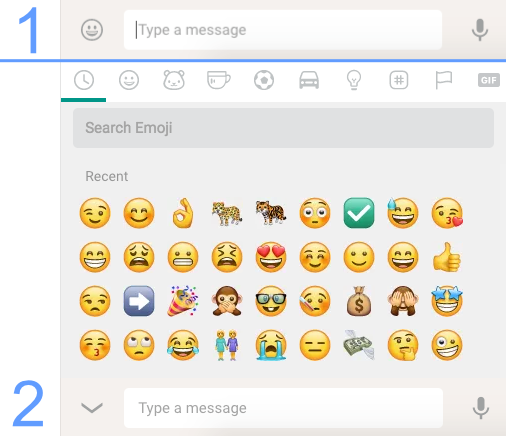
\includegraphics[width=\textwidth]{emojipasswords/whatsapp-picker-steps}
		\caption{\label{fig:emojipasswords:whatsapp-point-and-click}Two-step point-and-click interface  in WhatsApp.}
	\end{subfigure}
	\begin{subfigure}[t]{0.49\textwidth}
		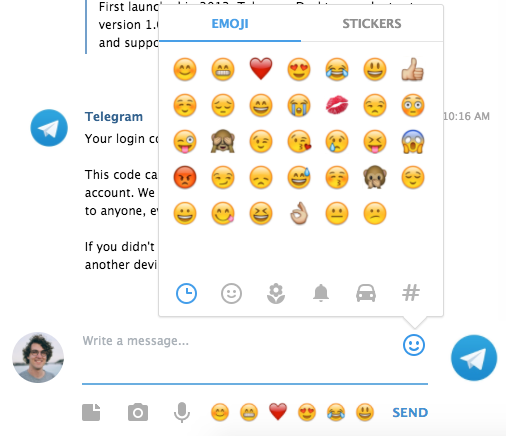
\includegraphics[width=\textwidth]{emojipasswords/telegram-picker}
		\caption{\label{fig:emojipasswords:telegram-point-and-click} Telegram shows the picker after the user hovers  the emoji button. Moreover, recently used emojis are shown beneath the text-field.}
	\end{subfigure}
	
	\caption{\label{fig:emojipasswords:real-world-pickers}
		Examples for point-and-click interfaces (``emoji picker''). \textit{Progressive disclosure} is used to access
		the list of available emojis: The user first needs to interact with a control element (emoji button) or start typing a special character (mostly ``:''), before an emoji can be selected by clicking or auto-completion of the shortcode. The emoji is then inserted into the text field.
	} 
\end{figure}
% general ways to do this.
% web-based
The project focused on using emoji-passwords on web sites, therefore we built a web-based prototype with standard technologies (PHP, HTML5, JavaScript). We identified two solutions to enter emojis on a desktop computer: via a point-and-click interface, and ``shortcodes''. Most web-versions of messenger applications, e.g. WhatsApp Web, Telegram Web, Hangouts, etc., use the point-and-click approach (see Figure \ref{fig:emojipasswords:real-world-pickers}). A few communication tools also allow entering a predefined word that is then translated into an emoji. This \textit{shortcode} often needs to be put into braces, e.g. (smile) on Skype, or stand between to colons, e.g. :smile: on Slack (see Figure \ref{fig:emojipasswords:slack-emoji-interaction}). We implemented a prototype based on point-and-click selection and Slack-style shortcodes. However, shortcodes were not auto-completed, which is generally discouraged for passwords \cite{Melicher2016UsabilityMobileTextPasswords} and there was no ``recent emoji'' feature. 
% passwords show in clear text below the input field to verify their selection.
After clicking an emoji, the prototype did not use the unicode character inside the password field for technical reasons\footnote{emojis typically break the masking of password fields, because their encoding differs in byte-size}. Instead, the shortcode was automatically inserted and masked. To allow checking the entered password, it was displayed in plain text beneath the input fields (see Figure \ref{fig:emojipasswords:policy-memo-instruction}). 

% reduced set of 50 emoji.
While unicode v11.0 contained 2789 emojis\footurl{https://unicode.org/emoji/charts/full-emoji-list.html}{08.03.2018}, our prototype included a subset of 50 for several reasons. First, we found through iterative testing that there was a selection bias, if the full range of emojis was offered; testers mostly included emojis from the first page. Randomizing the order is counterproductive in terms of usability. Second, Golla \etal used a similar approach for their EmojiAuth system \cite{Golla2017EmojiAuth, Kraus2017Emoji}. Last, it very likely facilitates recognition, potentially increasing memorability of the emoji-password.

% available emojis: 14 people and smileys, 7 nature and animals, 6 foods, 5 activity, 6 objects, 7 symbols.
The 50 emojis were selected with certain features in mind. To evaluate issues arising from similarity, around a third of emoji should resemble another in the set. Fragmentation issues during authentication can only be seen for emojis whose appearance strongly differs on other platforms. Moreover, the emojis should appeal to users, e.g. because they are familiar with them. To achieve this, different emoji-categories should be respected. Consequently, we identified 50 suitable candidates from the most-used emojis on twitter\footurl{http://emojitracker.com/}{08.06.2018} from multiple categories: \textit{smileys \& people} (14), \textit{animals \& nature} (7), \textit{food and drink} (6), \textit{activities} (5), \textit{objects} (6), and \textit{symbols (7)}. We opted to include more smileys, because this roughly 50\% of unicode emoji characters fall into this category. Our emoji-picker randomly arranged the emojis in a 10x5 grid to isolate selection-by-position effects. 

% emojis: iOS 9.3, b/c WhatsApp used these on all platforms at the time (most commonly used messenger app in DE)
The prototype allowed to switch the rendered version of the emojis. For the purpose of the study, we only needed two separate types. The default version was based on the emojis from iOS 9.3 (see Figure \ref{fig:emojipasswords:ui-open-picker}). This default was chosen, because WhatsApp used the same emoji-style across all platforms at the time of the study. Thus, we could expect participants to be familiar with them. The second style was based on Android 7.0 (``blob emojis''\footurl{https://medium.com/google-design/redesigning-android-emoji-cb22e3b51cc6}{08.03.2018}). 

\begin{figure}
	\centering
	\begin{subfigure}[t]{0.49\textwidth}
	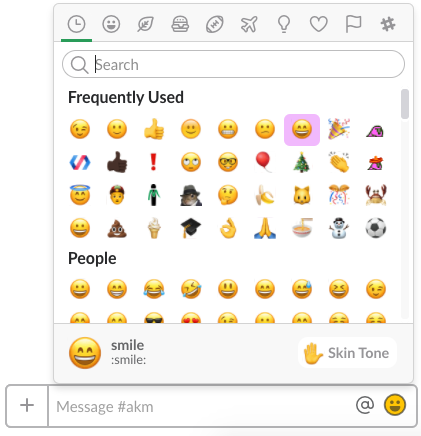
\includegraphics[width=\textwidth]{emojipasswords/slack-picker-shortcode}
	\caption{\label{fig:emojipasswords:slack-picker} The picker shows the short-code of the emoji for future use.}
	\end{subfigure}
	\begin{subfigure}[t]{0.49\textwidth}
	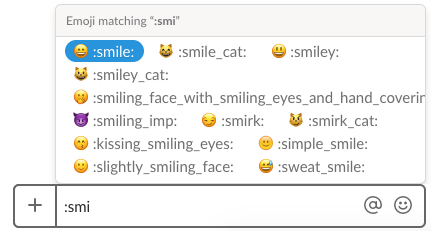
\includegraphics[width=\textwidth]{emojipasswords/slack-shortcode-auto}
	\caption{\label{fig:emojipasswords:slack-picker-shortcode} The user can guess the shortcode. Slack offers matching emojis.}
	\end{subfigure}
	\caption{\label{fig:emojipasswords:slack-emoji-interaction}
		Slack allows the user to utilize both a point-and-click interface and shortcodes to enter emoijs.
	} 
\end{figure}


\subsection{Password Selection in the Lab}
For the first part, participants were invited to a lab at the media informatics research group. The primary task was to create a password that participants could remember. There was no independent variable for the password selection task, thus participants all received the same study instructions. 

\subsubsection{Metrics}
% no clear-text passwords, emojis and zxcvbn stats, hashes are stored for verification purposes.
We logged the chosen emojis and their positions inside the passwords. Moreover, we analyzed password characteristics with zxcvbn and stored this to the database along with the hashed password. 
% time
As an indicator for usability of either the picker or the shortcodes, we measured the time taken to select the password. Here, we used the ``focus'' and ``blur'' events as start and end points. 

% self-reported: (questionnaire) selection strategies, motivation, input type (motivation, ease of use, usefulness, 5 point scale)
On the qualitative side, we used ordinal five-point scales to collect attitudinal data about using emojis inside passwords, the picker and shortcodes. Demographic data and self-reported password behavior helped us put measurements into context. 
% think aloud protocol, exit interview.
Everything that participants said during the study was protocolled. 

\subsubsection{Procedure}
% PC self guided with aid of experimenter
% briefing and informed consent (log data will be generated from interactions).
After an in-depth briefing on the purpose of the study and data collection practices, an experimenter explained each step of the study. We provided a standard desktop PC to complete the tasks, which were mostly self-guided. First, participants created a user ID. 
% create user Id (algorithm first letter parents' namses, birthplace, birth month)
Since they were going to need this ID later on to allow us matching the lab and field data, we provided a simple algorithm to create an ID. Participants were asked to take the first letter of both their parents' first names and their own birth place, appended by the digit of their birth month (e.g. ``IKP10''). This algorithm, albeit not perfectly random, was sufficient to protect personally identifiable information (PII).

This was followed by a questionnaire on demographic data, password coping strategies and attitudes towards emojis in passwords, e.g. ``\textit{how likely would you consider using emojis in a password?}'' At this point of the study, participants had not yet created an emoji-password, so their attitudes were not biased by later tasks. 
% instruction: difference between emojis and emoticons (shared understanding)
We also briefed them about the difference between ``emojis'' and ``emoticons'' to avoid misinterpretation. 

% password selection & commitment (think aloud)
% scenario: whatsapp requires all users to secure their account with a password (basic8 + emoji, feedback provided when policy is met.) 
Afterwards, participants completed the password selection task using the prototype. A significant part of the screen was dedicated to list all emojis and their short codes. To provide sufficient background information and introduce a realistic risk \cite{Krol2016ExperimentDesign}, the task included a scenario. It asked participants to imagine that they had used WhatsApp for some time and now a new security precaution is introduced. As a safety measure, they were now required to prove their identity with a password upon activating WhatsApp on a new device. The password needs to consist of at least eight alphanumeric characters and at least one emoji. 
% repeat password, only proceed if confirmed to have memorized the password.
Participants then had to repeat the selected password, and tick a box to confirm that they had memorized it (see Figure \ref{fig:emojipasswords:policy-memo-instruction}). 
% usability rating (picker/short codes, emoij-password concept post experience)
This was followed-up through a reflective self-assessment of their behavior during the study (cf. \cite{Fahl2013EcologicalValidityPasswordStudy}), and a structured questionnaire on their selection strategies. 

% interpretation task 
The study concluded with an interpretation task of two given emojis, namely the ``information desk person'' (\emoji{1F481}) and ``folded hands'' (\emoji{1F64F}). Those were not available during password selection, and we intended to assess their suitability for future inclusion. In total, the whole session duration was below 15 minutes.

\begin{figure}
	\centering
	\begin{subfigure}[t]{0.49\textwidth}
		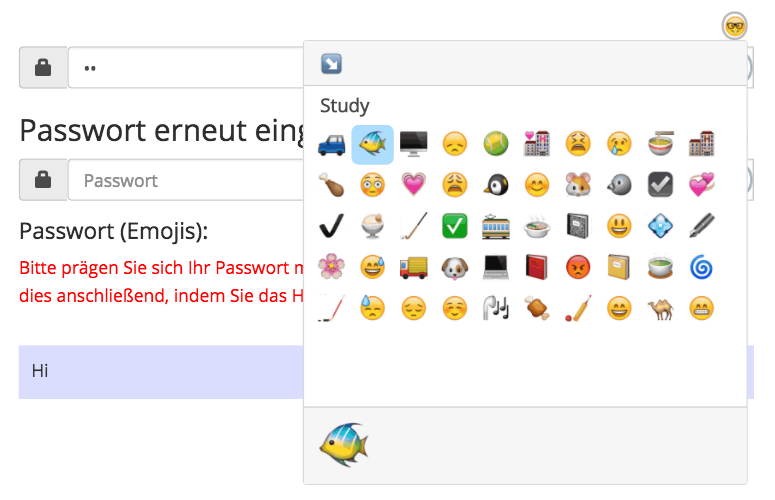
\includegraphics[width=\textwidth]{emojipasswords/open-picker}
		\caption{\label{fig:emojipasswords:ui-open-picker} Point and click interface. It is opened by clicking on the \emoji{1F913} button. The order of emojis is randomized. Upon selecting an emoji, it automatically closes.}
	\end{subfigure}
	\begin{subfigure}[t]{0.49\textwidth}
		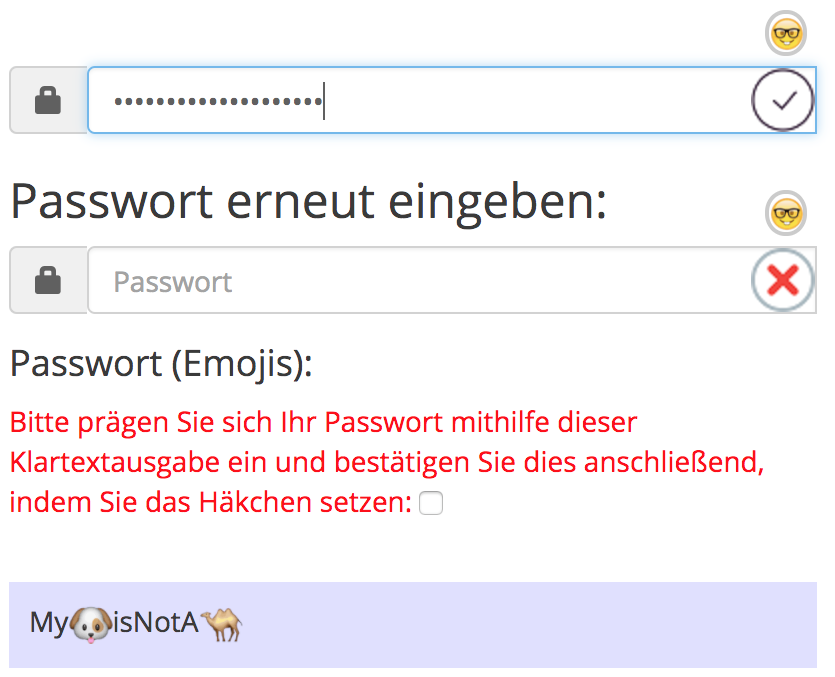
\includegraphics[width=\textwidth]{emojipasswords/ui-slim_cropped-2}
		\caption{\label{fig:emojipasswords:policy-memo-instruction} Screenshot of the user study. The selected password needed to be re-created. Additionally, participants need to tick a check-box to confirm that they had memorized their password.}
	\end{subfigure}
	\caption{\label{fig:emojipasswords:prototype} Prototype as used in the study.}
\end{figure}

% recall
\subsection{Unmoderated Remote Memorability Study}
% exactly one week after participant, invitation to return to the online study. 
Exactly one week after completing the first study part in the lab, participants were invited to return for the second round of tasks on-line. This primarily focused on memorability metrics and a reassessment of attitudes. 
\subsubsection{Independent Variables}
% emoji rendering (2 levels / degrees of freedom ): control group received iOS 9.3 (the same kind as in the lab), experimental group different treatment (Androd 7.0). 
To assess the influence of emoji fragmentation, we used one independent variable \textit{``rendering''} with two levels. For the \textit{control} group, emojis in the picker were rendered identically as before. In the experimental group, we replaced the iOS emojis with the Android 7.0 version. No other variations were made. 
\subsubsection{Dependent Variables}
% attempts to log in (max 3). 1 = immediate success, no errors.
We measured the number of attempts participants needed to log in. If they failed to log in on the first try, we counted this as an error.  Moreover, we collected memorization and recall techniques. 
% qual: how memorized? attitudinal ratings, qualitative feedback on overall technique
Finally, subjective usability ratings on the overall concept and qualitative feedback were gathered. This part of the study took about five minutes.

\subsubsection{Procedure}
% randomly put into the two treatment groups, different participation link for the two groups via email
Participants were randomly assigned to one of the two experimental groups. We emailed the corresponding link to the online study and requested completion within two days. 
% recreate user id same algorithm as in the lab)
The web page instructed them to recreate their user ID, providing the same algorithm as in the first part. Afterwards, participants were asked to log-in via their previously selected password. After unsuccessful attempts, the log-in counted as failed and the study proceeded automatically. However, as a memory support tool, we displayed the list of short codes after the first failed attempts. The study concluded with an attitudinal questionnaire about the perceived usability of the concept. 

\subsection{Recruiting and Demography}
We spread a registration link for a ``study on emojis'' via social networks and an official university newsletter. A 5€ shopping voucher served as incentive. The study was announced to take around 15 minutes. 40 people were screened in and all showed up to their study appointment. All of them were students at the LMU, and aged between 19 and 44 ($M=23$).  %TODO add standard deviation. (if we have it)
Users in this age rage are most likely to use emojis on a regular basis \cite{EmogiResearch2016}. 39 participants returned for the second study part on-line. The control group was formed by 20 participants, and the experimental group by 19. 


% announced as ``entering emojis and passwords''

\section{Results}
\subsection{Emoji Selection}
% quant:
% 	which emoijs were selected (distribution graph like on slides)
% 	position in password -> new graph (R!), with data from slides.
% qual:
% 	selection strategies
\subsection{Input Methods}
% quant: 
% 	how many used what
% qual:
%	why? feedback, sentiment.
\subsection{Memorability and Recognition}
% quant: 
%	how many succeeded? which emojis were involved in errors? group differences
% 	show the differences visually (like google talk)
% qual:
%	noticed differences?
%	how did people remember? memorization strategies
%	was the short code useful?

\subsection{Interpretation Task}
% basically what we wrote in the paper to illustrate that already for two given emojis there is a huge range of possible interpretations.

\subsection{Attitudes}




\subsection{Limitations}
% small sample size, homogeneous --> primary user group who are most likely to adopt emojipws as first-movers.
% ecological validity, self-report, novelty effects --> concrete plausible scenario, no reason not to trust P's.
% no attack vectors, only usability, behavioral, attitudinal data --> future work, but maybe compare to the advantage of adding a Xclass requirement over X-1class requirement from another study. that should do. 

\section{Discussion}

\subsection{Selection Strategies}
% what did they focus on? --> memorability, not security
% what does that mean?
% does that help?

% covariate: personality? \cite{Marengo2017EmojiPersonality}

\subsection{Fragmentation Issues}
% not yet crystal clear.


\subsection{Input UX}
% was it troubling? no
% does that mean, that all password fields on desktops should be accompanied by 
% of course entering an emojipw takes longer. even reading a text that includes emoji takes longer \cite{Gustafsson2017EmojiReadingTIme}


\section{Conclusion}
% services have started allowing the full unicode character set inside password. and it makes sense, especially because generated passwords can take a much richer character set (although it's not really necessary because )

% future work:
% strength,
% observability

\section{Take-Aways}
